% Appendix A

\chapter{Caso de estudio: SAT}
\label{apendiceB}
\lhead{Apéndice B. \emph{Caso de estudio: SAT}}

En este sección se considera un problema pequeño de SAT y se describe el
procedimiento de traducción y obtención de un plan.
La instancia de SAT que se resolverá es
\begin{equation}
(p \lor \neg q \lor r) \land (\neg p \lor \neg r) \land (\neg p \lor q).
\end{equation}

\section{Dominio}
\subsection{Entrada}
La modelación del dominio SAT fue descrita en la sección
\ref{modelacionproblemas}. Utilizando el lenguaje lógico que se ha definido en
este capítulo, tenemos que $\Phi_\SAT$ es:
\begin{verbatim}
(so-exists (?T 1) (forall (?y) (exists (?x)
      (or (and (?P ?x ?y) (?T ?x)) 
          (and (?N ?x ?y) (not (?T ?x)))))))
\end{verbatim}

La firma $\sigma_\SAT$ consta de las relaciones $N$ y $P$, las cuales 
varían de instancia a instancia y definen las cláusulas CNF del problema.

\subsection{Salida}
La herramienta crea el árbol sintáctico de $\Phi_\SAT$, el cual se muestra en
detalle en la Figura \ref{arbolsintactico}, y genera el archivo PDDL que se
presenta a continuación.

\begin{verbatim}
(define (domain SAT)
  (:constants zero max)

  (:predicates
    (es_cierto_conjuncion_2 ?x ?y) (es_cierto_conjuncion_6 ?x0 ?x1)
    (es_cierto_existencial_8 ?x0) (es_cierto_universal_9 ?x0)
    (es_cierto_disyuncion_7 ?x0 ?x1) (es_cierto_meta)
    (N ?x ?y) (P ?x ?y) (T ?x) (no-T ?x)
    (SUC ?x ?y)
  )
\end{verbatim}

El encabezado del archivo enumera las proposiciones del problema de
planificación.

\begin{verbatim}
  (:action colocar_verdadera_T
    :parameters (?x)
    :precondition (and (conjetura) (no-T ?x))
    :effect (and (T ?x) (not (not-T ?x))))
\end{verbatim}

La acción \texttt{colocar\_verdadera\_T} establece que su parámetro de entrada
$x$, una variable proposicional, se considerará \textbf{verdadera} en la
construcción de la prueba. Si esta acción no se aplica sobre una variable
proposicional, se asume el caso contrario (la variable es falsa), como es
descrito en la sección \ref{simplificacion}.

\begin{verbatim}
  (:action empezar-prueba
    :precondition (conjetura)
    :effect (and (prueba) (not (conjetura)))) )
 \end{verbatim}

La acción \texttt{empezar-prueba} es necesaria para que el planificador pase de la fase
de conjetura a la fase de construcción de la prueba utilizando los valores de
$T$ previamente escogidos.

\begin{verbatim}
  (:action probar_conjuncion_6
    :parameters (?x ?y)
    :precondition (and (prueba)
                       (N ?x ?y) (not-T ?x))
    :effect (es_cierto_conjuncion_6 ?x ?y))

  (:action probar_conjuncion_2
    :parameters (?x ?y)
    :precondition (and (prueba)
                       (P ?x ?y) (T ?x))
    :effect (es_cierto_conjuncion_2 ?x ?y))
\end{verbatim}

Arriba se muestra la traducción de las dos subfórmulas más internas. Establecer
una conjunción de dos proposiciones se logra al comprobar que ambas son ciertas
por separado. Nótese que se agrega la proposición \texttt{prueba} como
precondición, por lo que la acción \texttt{empezar-prueba} debe ejecutarse
antes que cualquiera de estas acciones.

\begin{verbatim}
  (:action probar_disyuncion_7_0
    :parameters (?x ?y)
    :precondition (and (prueba)
                       (es_cierto_conjuncion_2 ?x ?y))
    :effect (es_cierto_disyuncion_7 ?x ?y))

  (:action probar_disyuncion_7_1
    :parameters (?x ?y)
    :precondition (and (prueba)
                       (es_cierto_conjuncion_6 ?x ?y))
    :effect (es_cierto_disyuncion_7 ?x ?y))
\end{verbatim}

Para probar la disyunción es suficiente probar cualquiera de sus operandos, en
este caso las conjunciones internas. Por esta razón se incluyen dos acciones
que agregan la proposición \texttt{es\_cierto\_disyuncion\_7}.

\begin{verbatim}
  (:action probar_existencial_8
    :parameters (?x ?y)
    :precondition (and (prueba)
                       (es_cierto_disyuncion_7 ?x ?y))
    :effect (es_cierto_existencial_8 ?x))

  (:action probar_universal_base_9
    :precondition (and (prueba)
                       (es_cierto_existencial_8 zero))
    :effect (es_cierto_universal_9 zero))

  (:action probar_universal_inductivo_9
    :parameters (?y1 ?y2)
    :precondition (and (prueba)
                       (SUC ?y1 ?y2)
                       (es_cierto_universal_9 ?y1)
                       (es_cierto_existencial_8 ?y2))
    :effect (es_cierto_holds_forall_9 ?y2))
\end{verbatim}

Las acciones que hacen la demostración de los operadores \textit{existencial} y 
\textit{para todo} se muestran arriba. Nótese como el planificador debe iterar
sobre todos los objetos para probar inductivamente el operador universal.

\begin{verbatim}
  (:action probar-meta
    :precondition (es_cierto_universal_9 max)
    :effect (es_cierto_meta))
\end{verbatim}

Finalmente, la última acción establece que el estado meta es alcanzable cuando
se haya demostrado el operador universal para el último objeto (es decir, para
todos).

\begin{landscape}
\begin{figure}[h!]
\centering
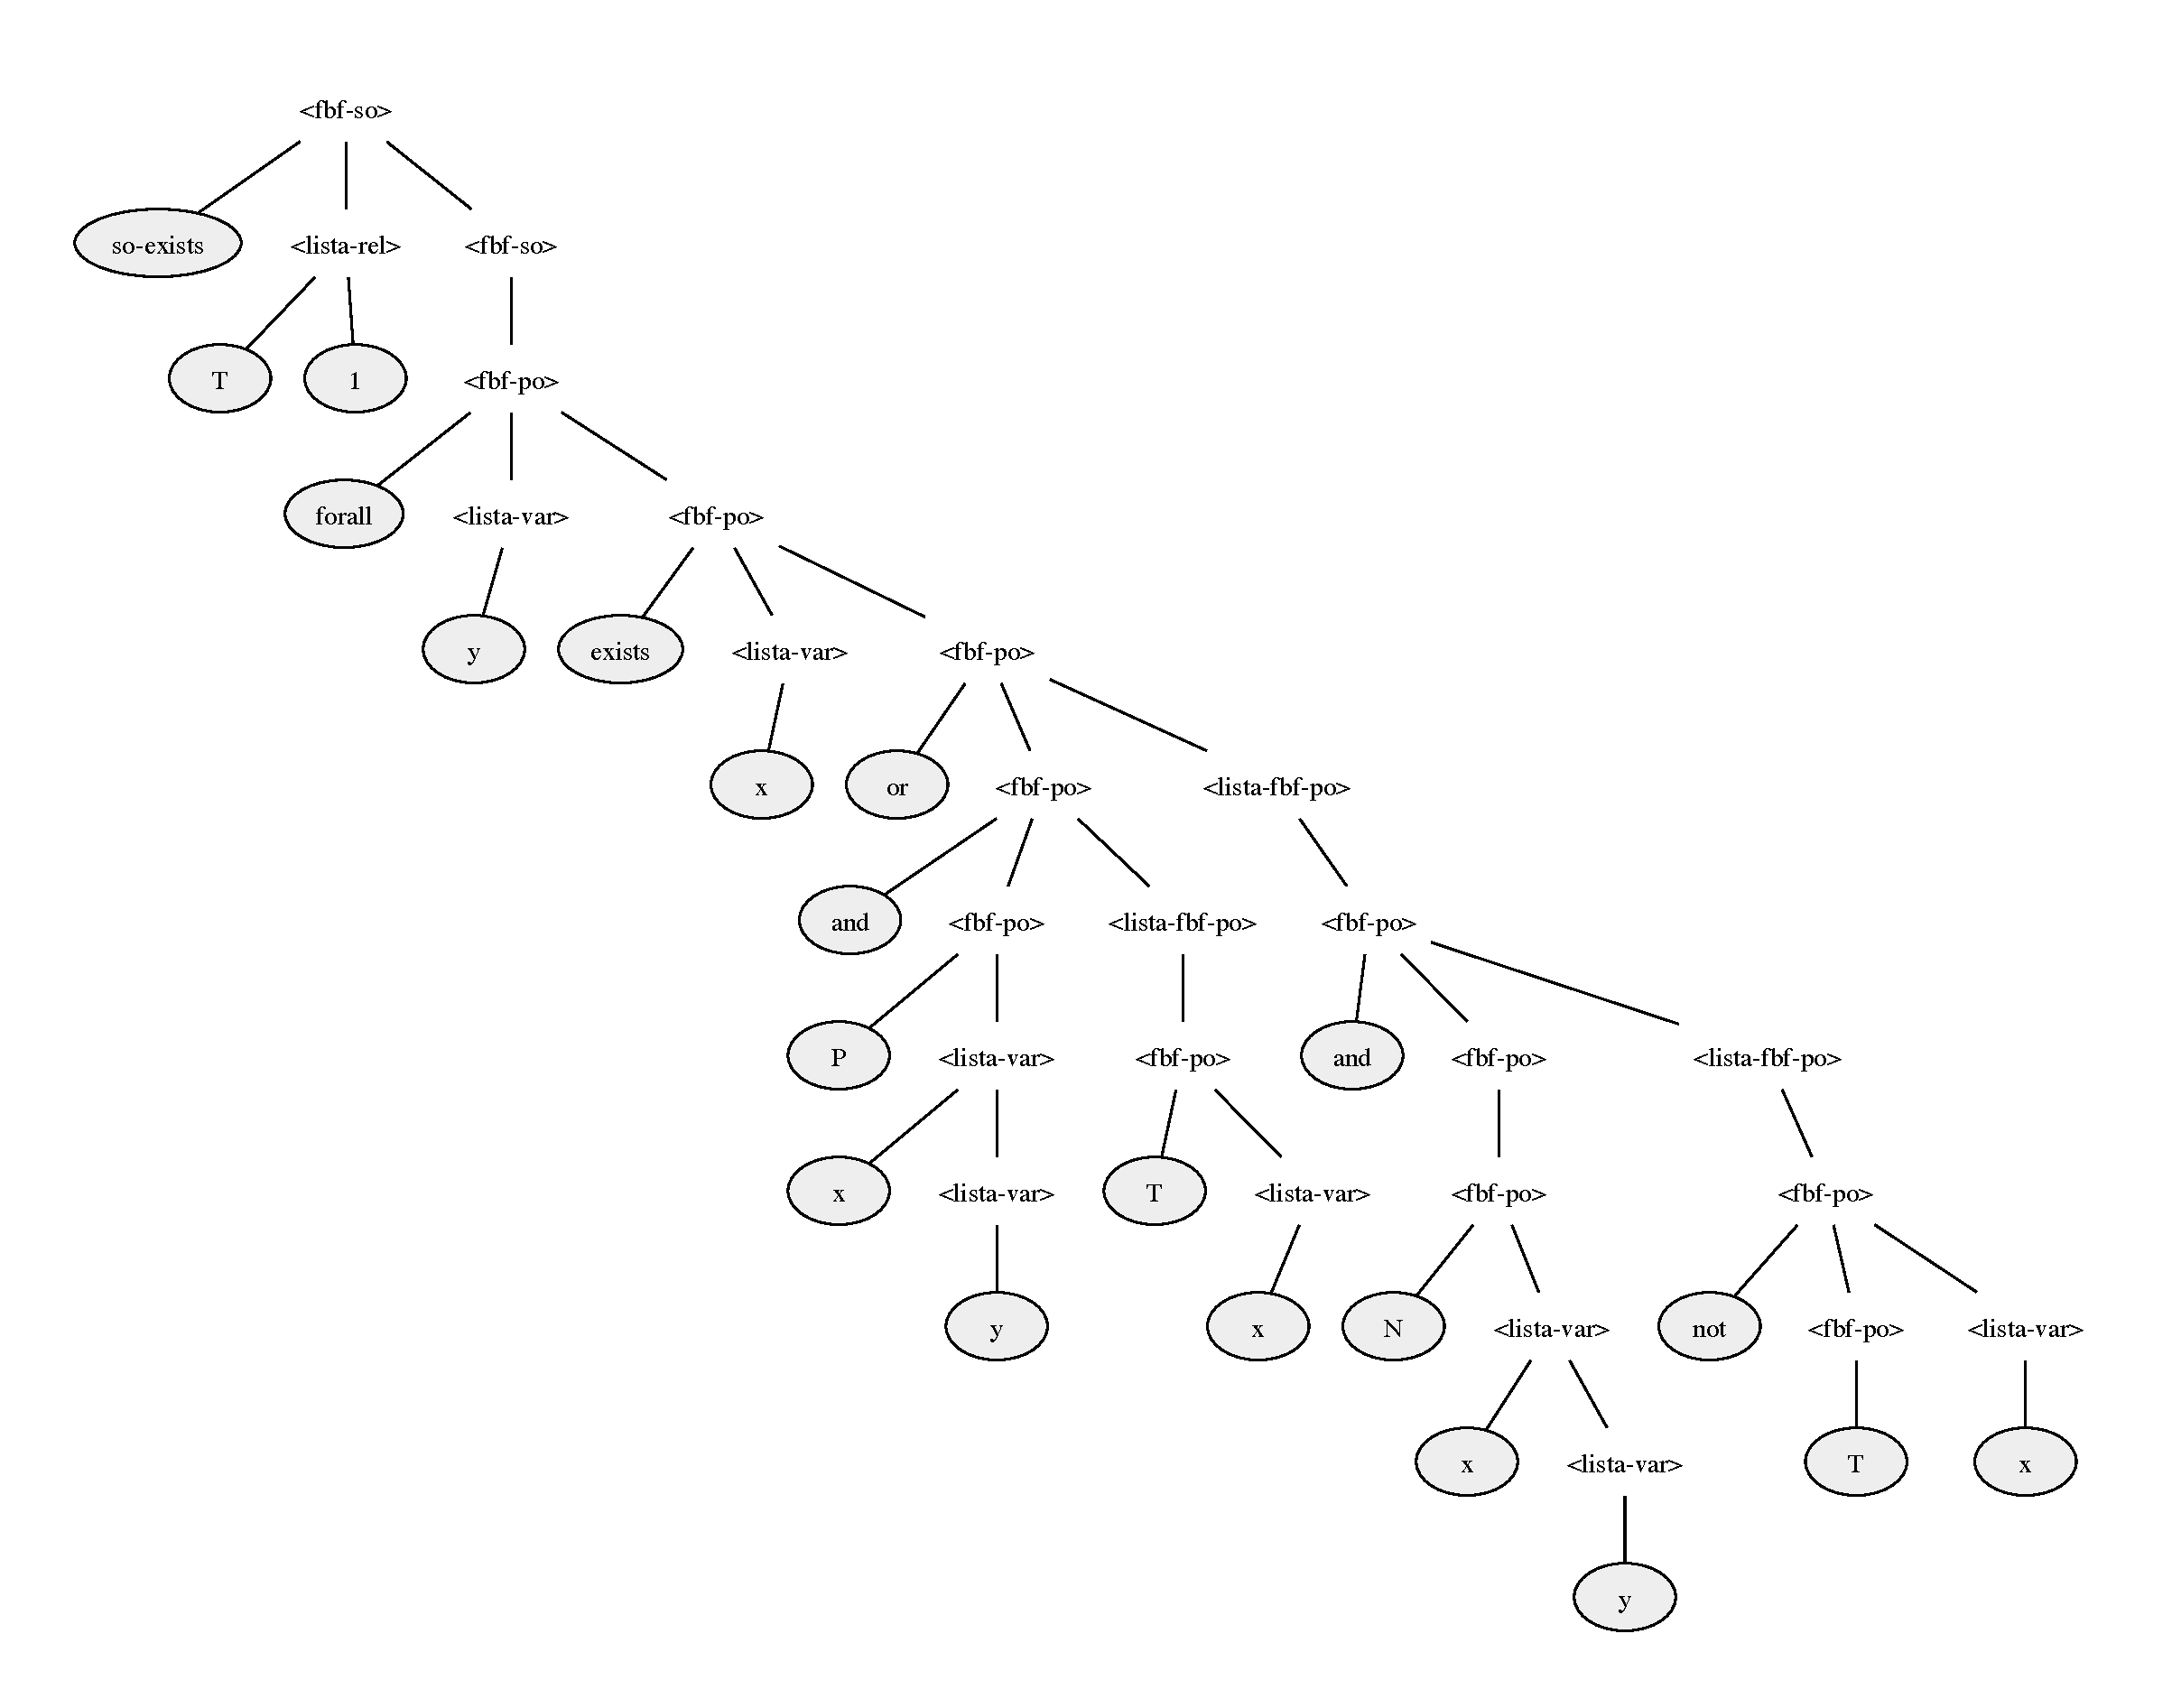
\includegraphics[height=\textheight]{figuras/arbolsintaxis.pdf}
\caption[Arbol sintáctico de $\Phi_{SAT}$]{Árbol sintáctico que construye el \textit{parser} al analizar la
sentencia $\Phi_{SAT}$. Los nodos terminales se marcan con un óvalo.}
\label{arbolsintactico}
\end{figure}
\end{landscape}

\section{Problema}
\subsection{Entrada}
La estructura finita que codifica la instancia descrita por la fórmula
B.1. es $\A = \tup{|\A| = \{\texttt{zero}, \texttt{obj1},
\texttt{max}\}, P, N}$, donde $P$ y $N$ son descritos con un archivo de texto
de entrada que contiene las líneas:

\begin{center}
\begin{verbatim}
; primera cláusula
(P zero zero)
(N obj1 zero)
(P max zero)

; segunda cláusula
(N zero obj1)
(N max obj2)

; tercera cláusula
(N zero max)
(P obj1 max)
\end{verbatim}
\end{center}

Esto codifica $(p \lor \neg q \lor r) \land (\neg p \lor \neg r) \land (\neg p
\lor q)$, con $p$ renombrada a \texttt{zero}, $q$ a \texttt{obj1}, y $r$ a
\texttt{max}.

\subsection{Salida}
La salida de la herramienta es el siguiente archivo PDDL que establece las
condiciones iniciales del problema:
\begin{verbatim}
(define (problem p)
    (:domain sat)
    ; zero y max fueron definidas como constantes del dominio
    (:objects obj1)
    (:init
        (guess)
        (SUC zero obj1)
        (SUC obj1 max)
        (not_t zero)
        (not_t obj1)
        (not_t max)
        (P zero zero)
        (N obj1 zero)
        (P max zero)
        (N zero obj1)
        (N max obj1)
        (N zero max)
        (P obj1 max)
    )
    (:goal (es_cierto_meta))
)
\end{verbatim}

\section{Solución}
Se utilizó M para hallar una solución al problema de planificación generado por
la herramienta. El plan encontrado fue el siguiente:
\begin{verbatim}
0 : (colocar_verdadera_T max)
1 : (colocar_verdadera_T obj1)
2 : (empezar-prueba)
3 : (probar_conjuncion_2 zero max)
4 : (probar_conjuncion_6 max zero)
5 : (probar_conjuncion_6 obj1 zero)
6 : (probar_disyuncion_7_0 zero max)
7 : (probar_disyuncion_7_1 max zero)
8 : (probar_disyuncion_7_1 obj1 zero)
9 : (probar_existencial_8 max zero)
10 : (probar_existencial_8 obj1 zero)
11 : (probar_existencial_8 zero max)
12 : (probar_universal_base_9)
13 : (probar_universal_inductivo9 zero obj1)
14 : (probar_universal_inductivo9 obj1 max)
15 : (probar-meta)
\end{verbatim}

La primera parte del plan, antes del operador \texttt{empezar-prueba}, es la
respuesta al problema de hallar una asignación de verdad a las variables $p$,
$q$ y $r$ que satisfaga la fórmula B.1. La asignación es $T =
\{\texttt{obj1}, \texttt{max}\}$, que es equivalente a $p = false$, $q = true$, $r = true$.
La segunda parte del plan muestra la demostración de que la asignación escogida
hace de $\Phi_\SAT$ una fórmula válida para la estructura de entrada.
